%%%%%%%%%%%%%%%%%%%%%%%%%%%%%%%%%%%%%%%%%
% Beamer Presentation
% LaTeX Template
% Version 1.0 (10/11/12)
%
% This template has been downloaded from:
% http://www.LaTeXTemplates.com
%
% License:
% CC BY-NC-SA 3.0 (http://creativecommons.org/licenses/by-nc-sa/3.0/)
%
%%%%%%%%%%%%%%%%%%%%%%%%%%%%%%%%%%%%%%%%%

%----------------------------------------------------------------------------------------
%	PACKAGES AND THEMES
%----------------------------------------------------------------------------------------

\documentclass[aspectratio=169]{beamer}

\mode<presentation> {

% The Beamer class comes with a number of default slide themes
% which change the colors and layouts of slides. Below this is a list
% of all the themes, uncomment each in turn to see what they look like.

%\usetheme{default}
%\usetheme{AnnArbor}
%\usetheme{Antibes}
%\usetheme{Bergen}
%\usetheme{Berkeley}
%\usetheme{Berlin}
%\usetheme{Boadilla}
\usetheme{CambridgeUS}
%\usetheme{Copenhagen}
%\usetheme{Darmstadt}
%\usetheme{Dresden}
%\usetheme{Frankfurt}
%\usetheme{Goettingen}
%\usetheme{Hannover}
%\usetheme{Ilmenau}
%\usetheme{JuanLesPins}
%\usetheme{Luebeck}
%\usetheme{Madrid}
%\usetheme{Malmoe}
%\usetheme{Marburg}
%\usetheme{Montpellier}
%\usetheme{PaloAlto}
%\usetheme{Pittsburgh}
%\usetheme{Rochester}
%\usetheme{Singapore}
%\usetheme{Szeged}
%\usetheme{Warsaw}

% As well as themes, the Beamer class has a number of color themes
% for any slide theme. Uncomment each of these in turn to see how it
% changes the colors of your current slide theme.

%\usecolortheme{albatross}
\usecolortheme{beaver}
%\usecolortheme{beetle}
%\usecolortheme{crane}
%\usecolortheme{dolphin}
%\usecolortheme{dove}
%\usecolortheme{fly}
%\usecolortheme{lily}
%\usecolortheme{orchid}
%\usecolortheme{rose}
%\usecolortheme{seagull}
%\usecolortheme{seahorse}
%\usecolortheme{whale}
%\usecolortheme{wolverine}

%\setbeamertemplate{footline} % To remove the footer line in all slides uncomment this line
%\setbeamertemplate{footline}[page number] % To replace the footer line in all slides with a simple slide count uncomment this line

%\setbeamertemplate{navigation symbols}{} % To remove the navigation symbols from the bottom of all slides uncomment this line
}

\usepackage{graphicx} % Allows including images
\usepackage{booktabs}% Allows the use of \toprule, \midrule and \bottomrule in tables
\usepackage[document]{ragged2e}
\usepackage{multirow}
\usepackage{adjustbox}
\usepackage{rotating}
\usepackage{enumitem}
\usepackage{pifont}
\usepackage{xcolor}
\usepackage{lmodern}


%----------------------------------------------------------------------------------------
%	TITLE PAGE
%----------------------------------------------------------------------------------------

\title[EE2023 - Technical Writing and Presentation]{Cyber-physical Infrastructure for Smart Building Applications towards Human Comfort and Energy Savings} % The short title appears at the bottom of every slide, the full title is only on the title page

\author[Tran Quang Anh 20212398]{Hoang Duc Chinh$^1$, S.S. Shinhu$^2$, K.R. Krishnanand$^3$, S.K. Panda$^2$}

 % Your name
\institute[HUST] % Your institution as it will appear on the bottom of every slide, may be shorthand to save space
{
$^1$Hanoi University of Science and Technology, Viet Nam \\
$^2$National University of Singapore, Singapore \\ % Your institution for the title page
$^3$Berkeley Education Alliance for Research in Singapore (BEARS), Singapore
\medskip
\textbf{\\ ISSN 1859-0551} % Your email address
}
\date[Instructor: Tran Thanh Son]{\small \textbf{Presenter:} Tran Quang Anh 20212398} % Date, can be changed to a custom date

\begin{document}

\begin{frame}
\titlepage % Print the title page as the first slide
\end{frame}

\begin{frame}{Overview} % Table of contents slide, comment this block out to remove it
\tableofcontents % Throughout your presentation, if you choose to use \section{} and \subsection{} commands, these will automatically be printed on this slide as an overview of your presentation
\end{frame}

%----------------------------------------------------------------------------------------
%	PRESENTATION SLIDES
%----------------------------------------------------------------------------------------

%------------------------------------------------
\section{Introduction} % Sections can be created in order to organize your presentation into discrete blocks, all sections and subsections are automatically printed in the table of contents as an overview of the talk
%------------------------------------------------

% \subsection{Subsection Example} % A subsection can be created just before a set of slides with a common theme to further break down your presentation into chunks

\begin{frame}{Introduction}
\begin{columns}
\column{0.5\textwidth}
    With development of IT:\\
    \begin{itemize}[label=$\circ$]
        \item Allow building integrated with \textbf{smart devices} and sub-system
        \item Increasing demand of \textbf{optimizing operation} to serve occupants needs
    \end{itemize}
    
    Solve problem of smart building application for \textbf{human confort} and \textbf{energy efficiency}:
    \begin{itemize}[label=$\circ$]
        \item \textbf{User-centric design} in creating truly smart buildings
        \item Utilizing cyber-physical system for optimal operation
    \end{itemize}

\column{0.5\textwidth}

\begin{figure}
    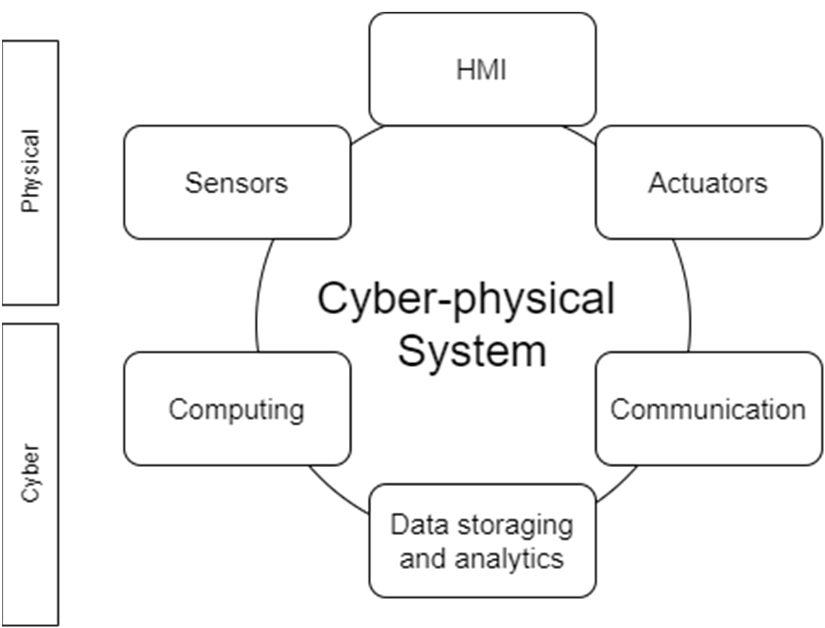
\includegraphics[scale=0.24]{pic/Cyber-Physical-system-key-characteristics.png}
    \caption{Cyber physical infrastructure}
    \label{fig:enter-label}
\end{figure}    
    
\end{columns}

\end{frame}

%------------------------------------------------



%------------------------------------------------

\section{Problem Statement and Approach}
\begin{frame}{Problem Statement}
\textbf{Wireless sensor and actuator networks (WSAN)} and IoT devices allow devices in building connects to others and users easily
\begin{figure}
    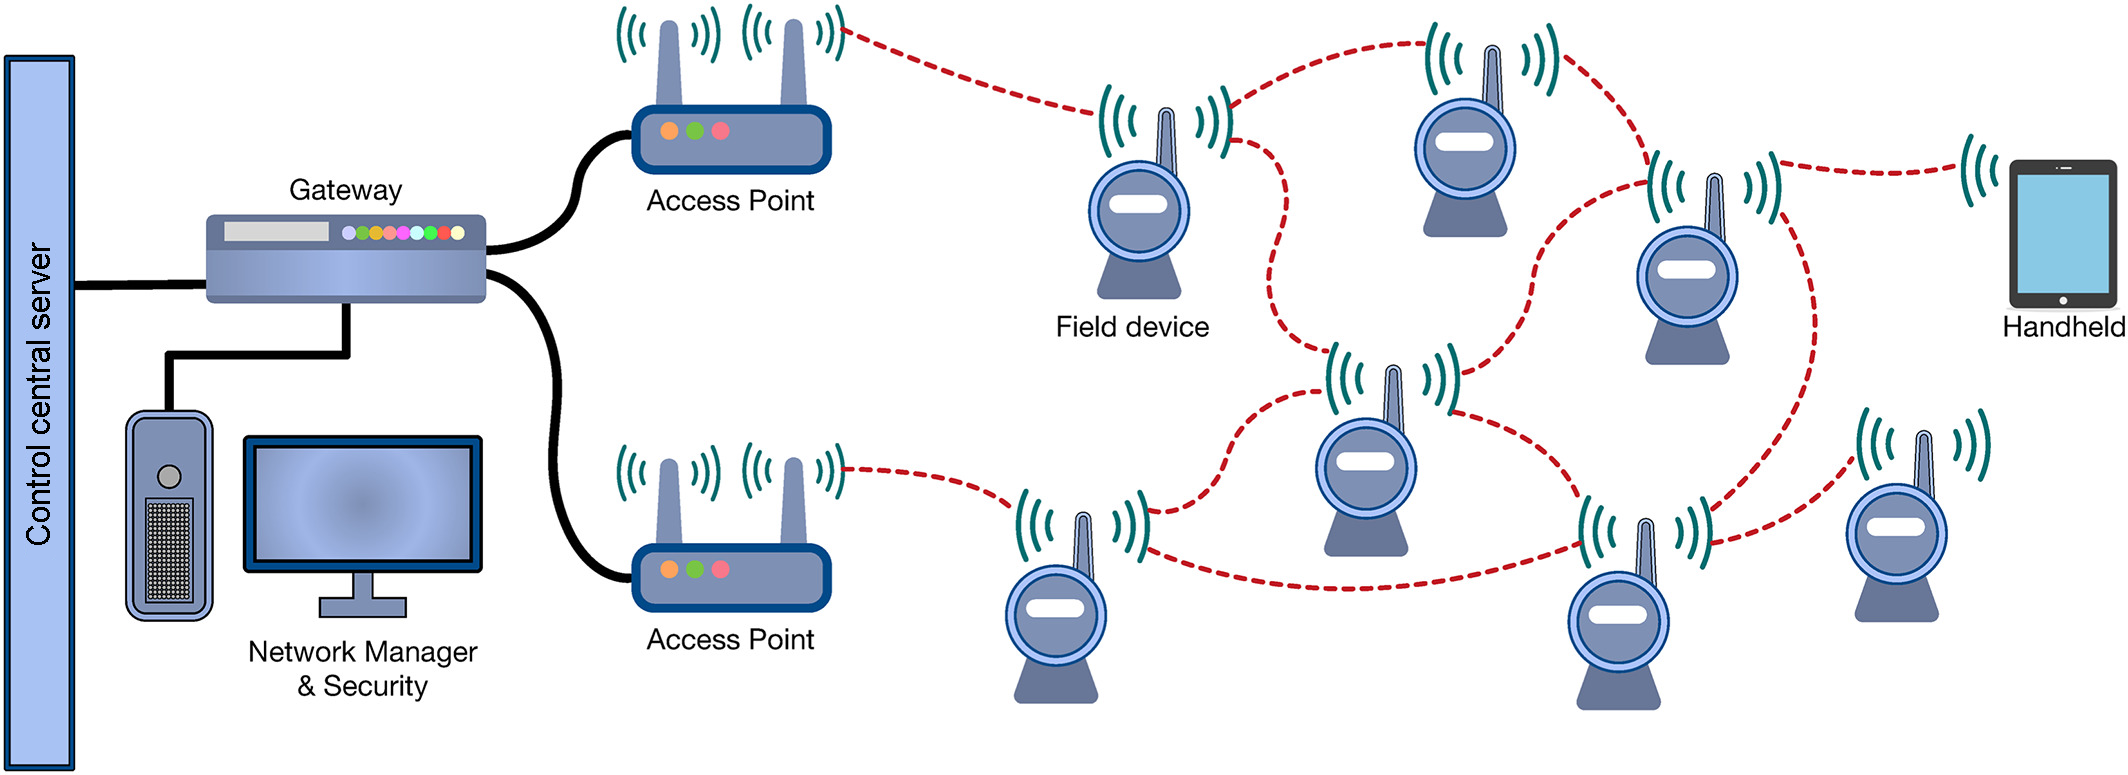
\includegraphics[scale=0.15]{pic/wsan.png}
    \caption{Wireless sensor and actuator networks (WSAN) and IoT systems}
\end{figure}
On the other hand, WSAN require many \textbf{\textcolor{red}{levels of integration}}, e.g., cross-technology integration or cross-organization integration
\end{frame}

\begin{frame}{Problem Statement}
    \textbf{Optimization} in energy efficiency may \textbf{limit human comfort}.\\~\\
    \textit{For example,} energy saving strategies \textbf{lack consideration} of \textbf{user control} and \textbf{personalized comfort}, or mainly determined through optimizing.\\~\\
    \begin{block}{}
        \textit{Problem \textbf{hardly} taken to account in \textbf{\textcolor{red}{conventional buildings}}, but a blind automation result in dissatisfaction or worse cases.}
    \end{block}
\end{frame}

\begin{frame}{Approach}
    \begin{columns}
        \column{0.5\textwidth}
        With \textbf{ubiquitous computing}:
        \begin{itemize}[label=$\circ$]
            \item Shifting building automation toward personalized and localized comfort
            \item Optimizing energy saving
            \item Requiring strong interconnected objects, devices and systems
        \end{itemize}

        \column{0.5\textwidth}
        \begin{figure}
            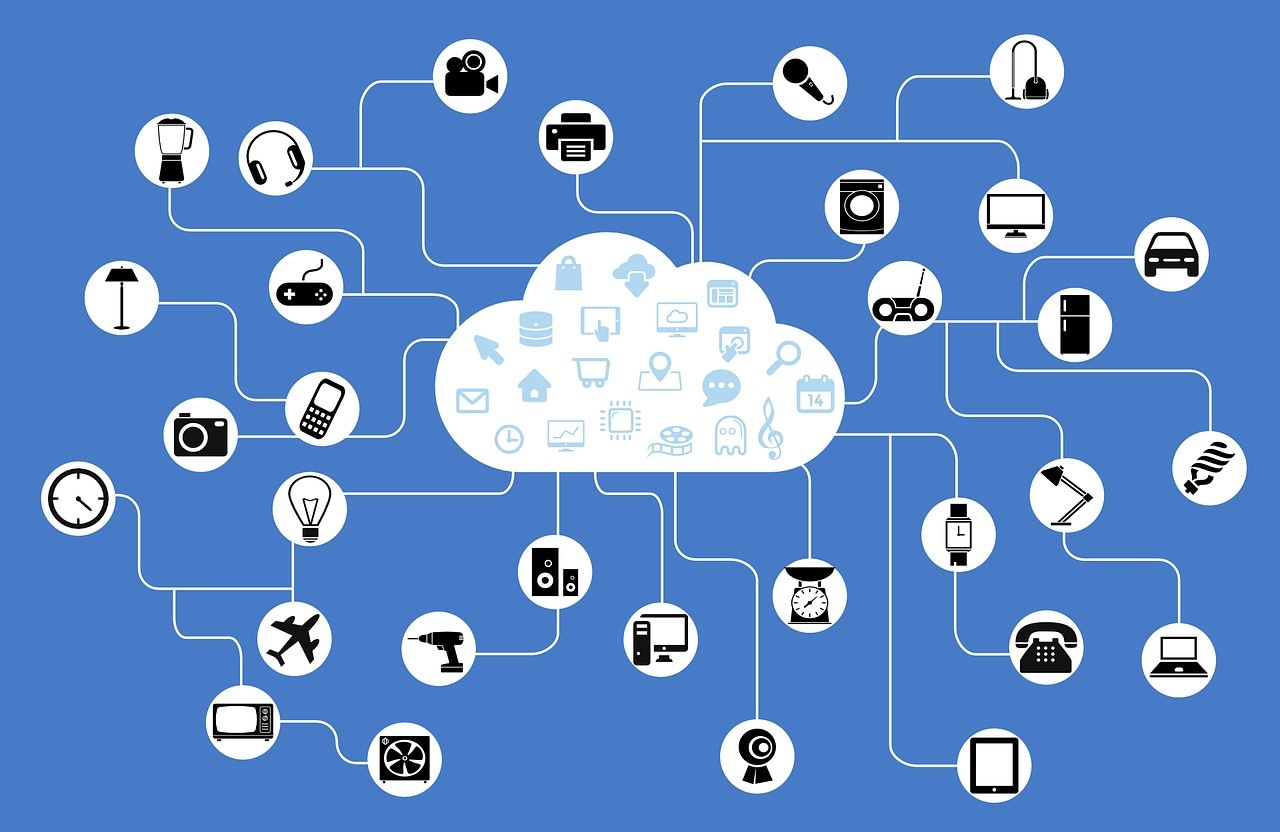
\includegraphics[scale=0.2]{pic/ubiquitous-computing-intro.jpg}
            \caption{\small{Ubiquitous computing}} 
        \end{figure}
    \end{columns}
\end{frame}

%----------------------------------------------------------------------------------------

\section{System Description}

\subsection{Hardware platform}
\begin{frame}{Hardware platform}
    Hardware platform consists of \textcolor{blue}{actuators}, wireless sensor networks and plug-load management.
    \begin{columns}
        \column{0.3\textwidth}
        \textbf{Actuator:}
        \small{
            \begin{itemize}[label=$\circ$]
                \item Using different communication protocols
                \item Supported by different hardware and software platforms
            \end{itemize}
        }
        
        \column{0.7\textwidth}
        \begin{figure}
            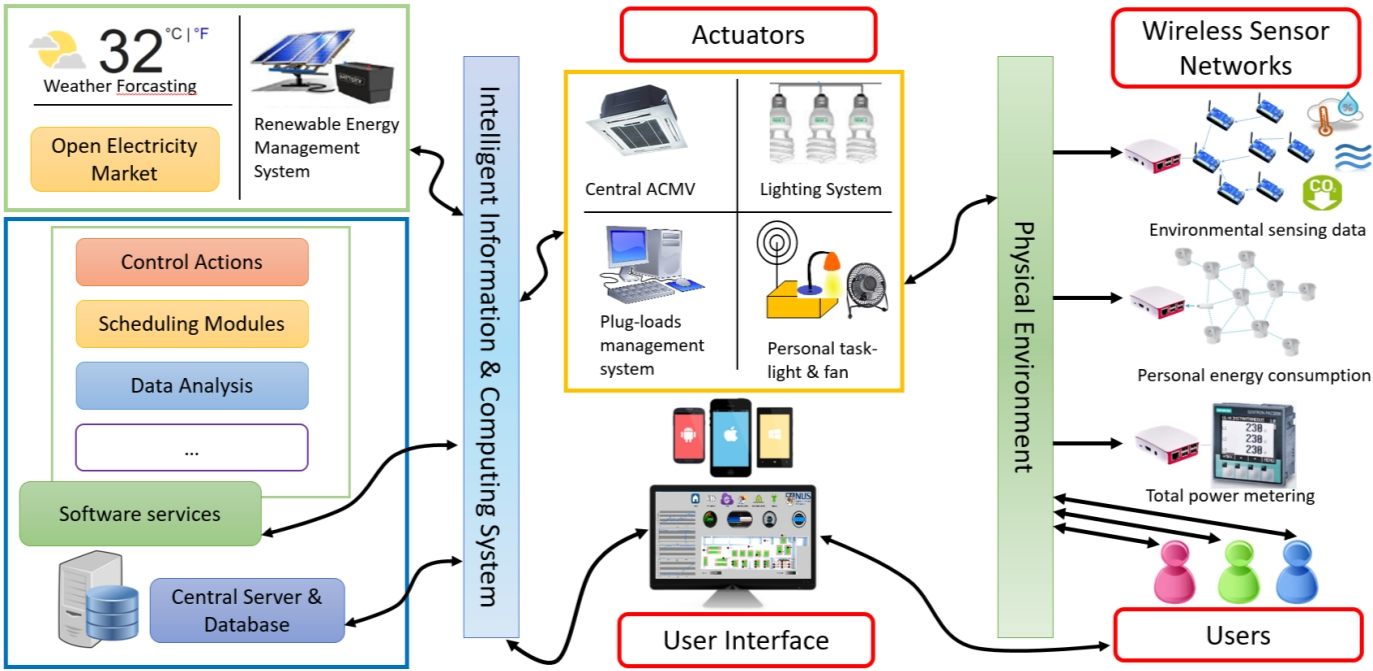
\includegraphics[scale=0.2]{pic/cyber-physical-infrastructure.png}
            \caption{\footnotesize{Cyber-physical system architecture with sub-systems and services}}
        \end{figure}
    \end{columns}
\end{frame}

\begin{frame}{Hardware platform}
    Hardware platform consists of actuators, \textcolor{blue}{wireless sensor networks} and plug-load management.
    \begin{columns}
        \column{0.3\textwidth}
        \textbf{Wireless sensor networks}
        \small{
            \begin{itemize}[label=$\circ$]
                \item Temperature, humidity, illuminance sensor boards (SBs) with Iris platform
                \item Zigbee-based Arduino board with CO2 sensor
                \item Raspberry Pi SBC equipped with communication module as gateways
            \end{itemize}
        }
        
        \column{0.7\textwidth}
        \begin{figure}
            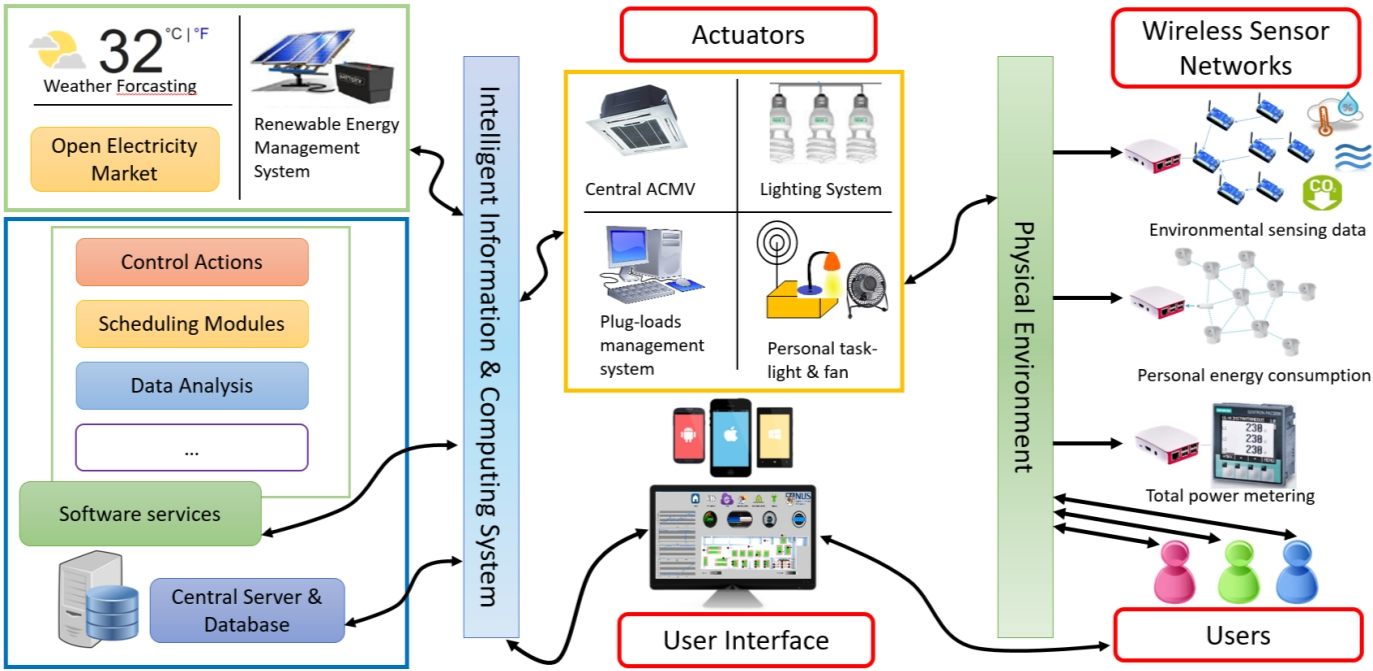
\includegraphics[scale=0.2]{pic/cyber-physical-infrastructure.png}
            \caption{\footnotesize{Cyber-physical system architecture with sub-systems and services}}
        \end{figure}
    \end{columns}
\end{frame}

\begin{frame}{Hardware platform}
    Hardware platform consists of actuators, wireless sensor networks and \textcolor{blue}{plug-load management}.
    \begin{columns}
        \column{0.3\textwidth}
        \textbf{Plug-load management:}
        \small{
            \begin{itemize}[label=$\circ$]
                \item Zigbee-based Plugwise power meters installed at each workspace 
                \item Siemen SENTRON PAC3200 total power monitoring meters using ModbusTCP protocol
            \end{itemize}
        }
        
        \column{0.7\textwidth}
        \begin{figure}
            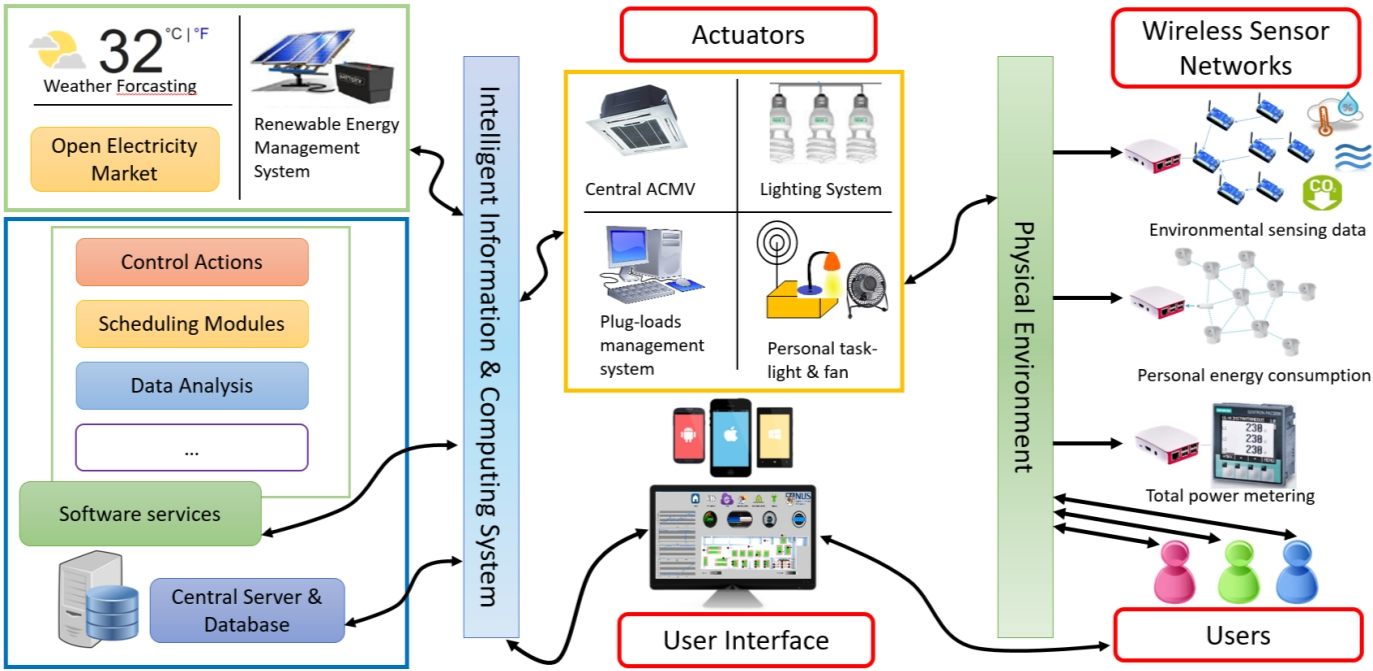
\includegraphics[scale=0.18]{pic/cyber-physical-infrastructure.png}
            \caption{\footnotesize{Cyber-physical system architecture with sub-systems and services}}
        \end{figure}
    \end{columns}
\end{frame}

\subsection{Software Development and System Deployment}
\begin{frame}{Software Development}
    Software system consists of modules at different levels:
    \begin{columns}
        \column{0.5\textwidth}
        \begin{small}
            \begin{block}{\textbf{Sensor-actuator node}}
                Perform sensing, actuating, communication tasks
            \end{block}
            \begin{block}{\textbf{Base station (gateways)}}
                \begin{itemize}[label=$\circ$]
                    \item Communicating with sensor-actuator nodes and central server
                    \item Storing, pre-processing local data or making control action decision
                \end{itemize}
            \end{block}
            \begin{block}{\textbf{Control central server}}
                Multi-threading application is run to deal with data stream from different base stations.
            \end{block}
        \end{small}

        \column{0.5\textwidth}
        \begin{figure}
            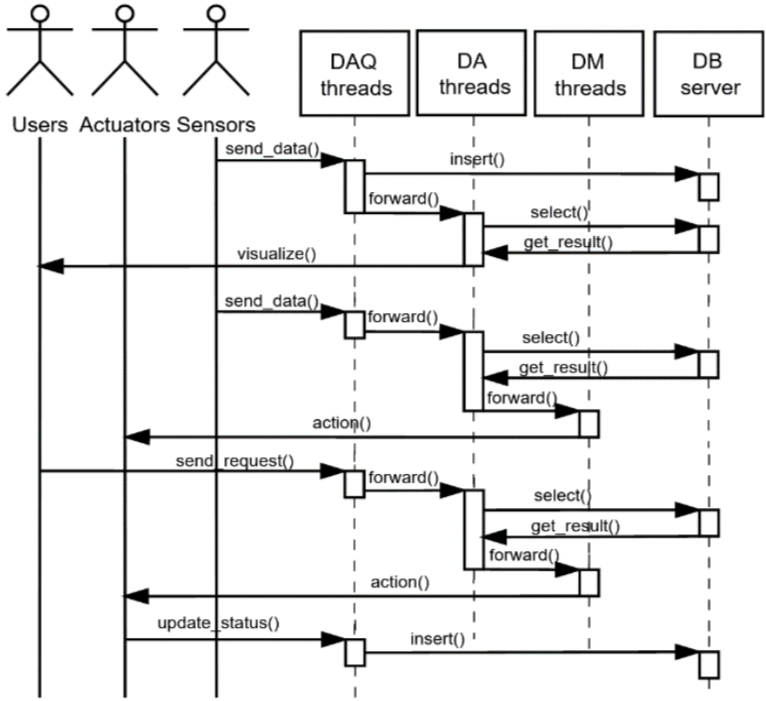
\includegraphics[scale=0.2]{pic/multi_thread.png}
            \caption{\footnotesize{Multiple threads of the main applications}}
        \end{figure}
    \end{columns}
\end{frame}

\begin{frame}{Database structure}
    \begin{columns}
        \column{0.55\textwidth}
        \begin{figure}
            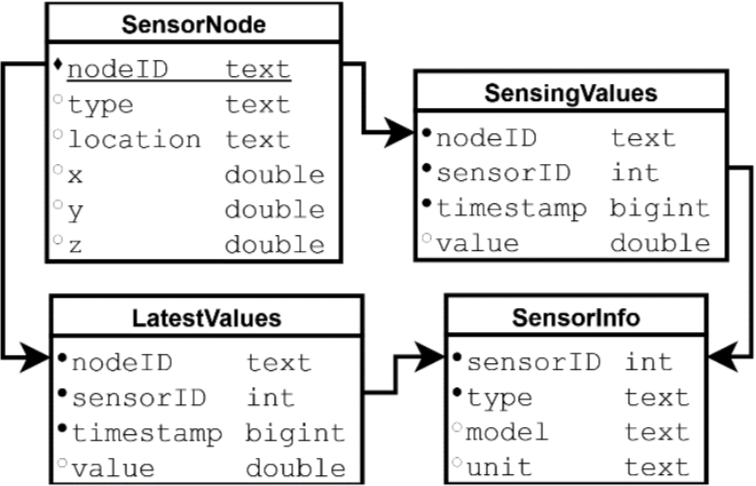
\includegraphics[scale=0.27]{pic/data-scheme.png}
            \caption{\footnotesize Database schema for storing collected values}
        \end{figure}

        \column{0.45\textwidth}
        \small{\begin{itemize}[label=$\circ$]
            \item \textit{\textbf{SensorValues:}} value from sensors and metadata table
            \item \textit{\textbf{LatestValues:}} data snapshot for quick access and visualization
            \item \textit{\textbf{Metadata:}} sensors' infomation
        \end{itemize}
        }
    \end{columns}
\end{frame}

\begin{frame}
    \frametitle{System deployment}
    \begin{figure}
        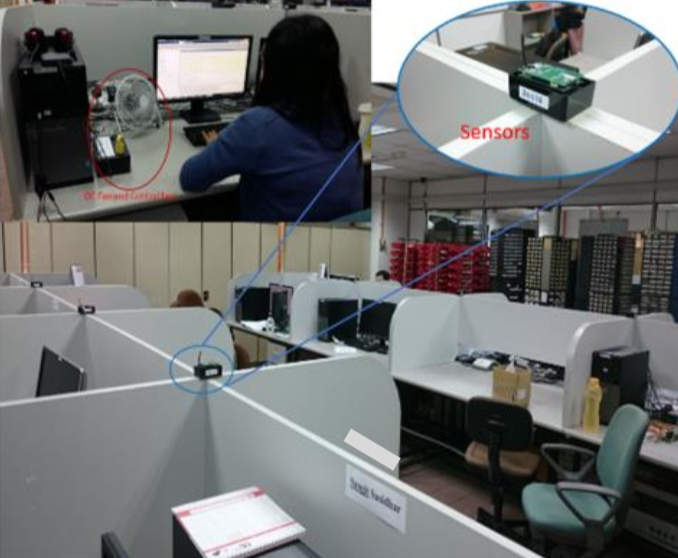
\includegraphics[scale=0.25]{pic/office.png}
        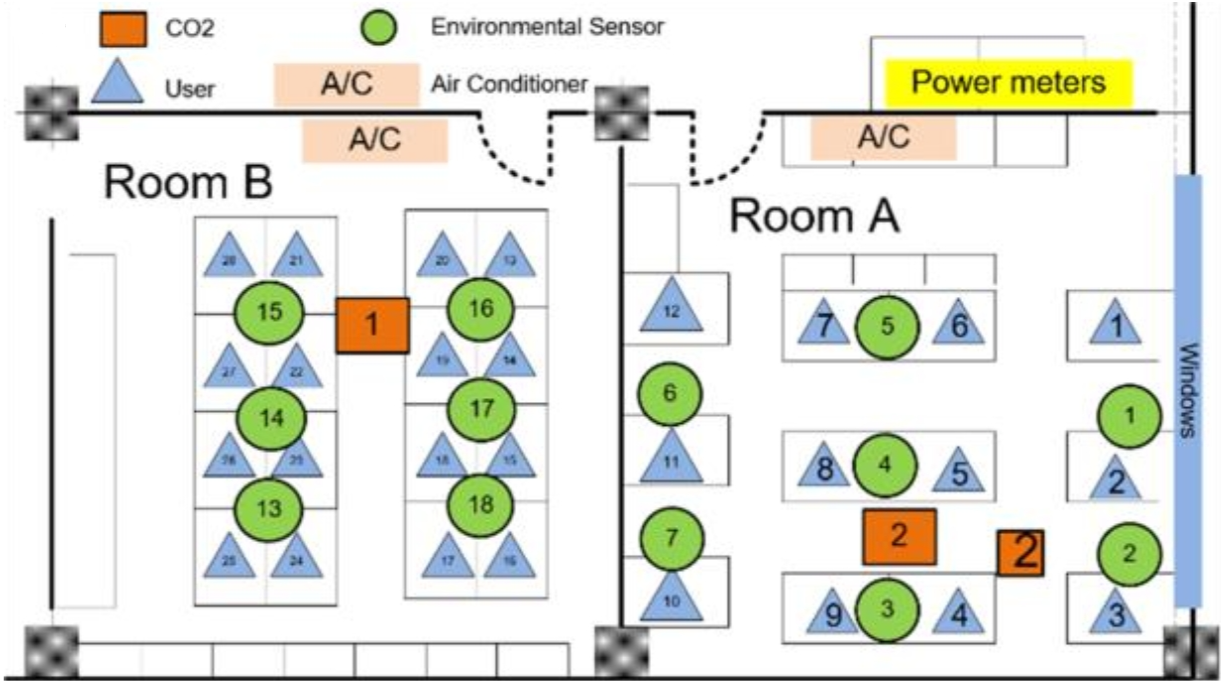
\includegraphics[scale=0.2]{pic/system_deployment.png}
        \caption{Device deployments in a shared office area}
    \end{figure}
\end{frame}

%==================================

\section{Data Analysis and Discussion}
\begin{frame}
    \frametitle{Data analysis}
    \begin{figure}
        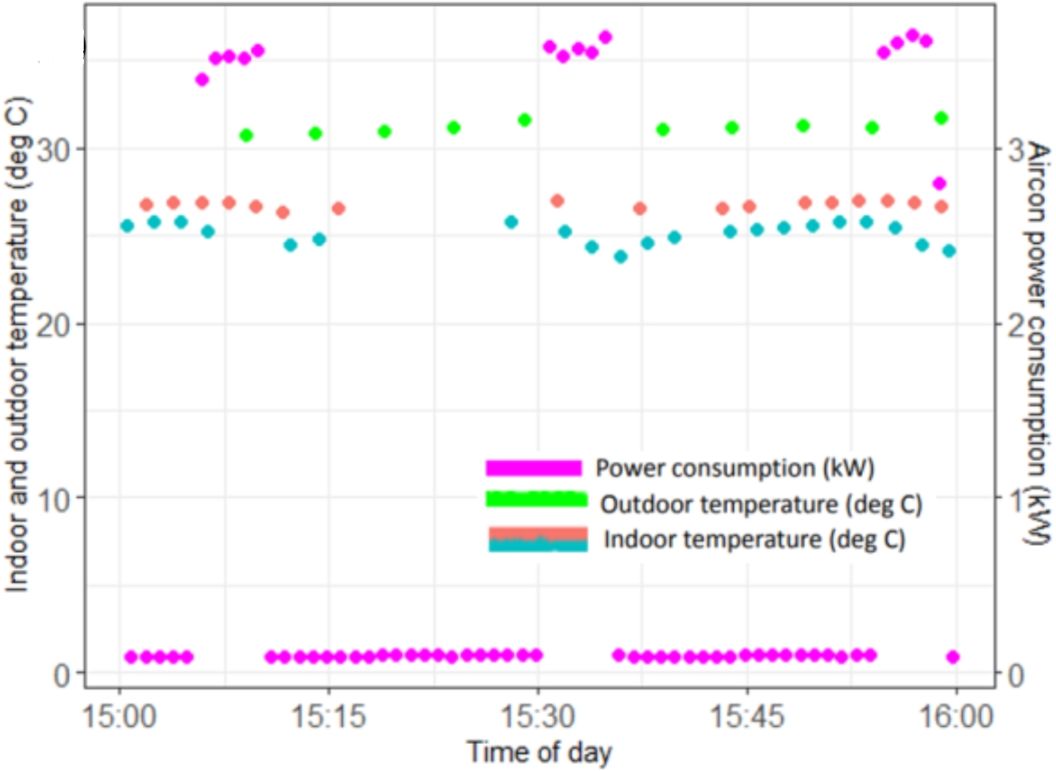
\includegraphics[scale = 0.19]{pic/ac_power_A.png}
        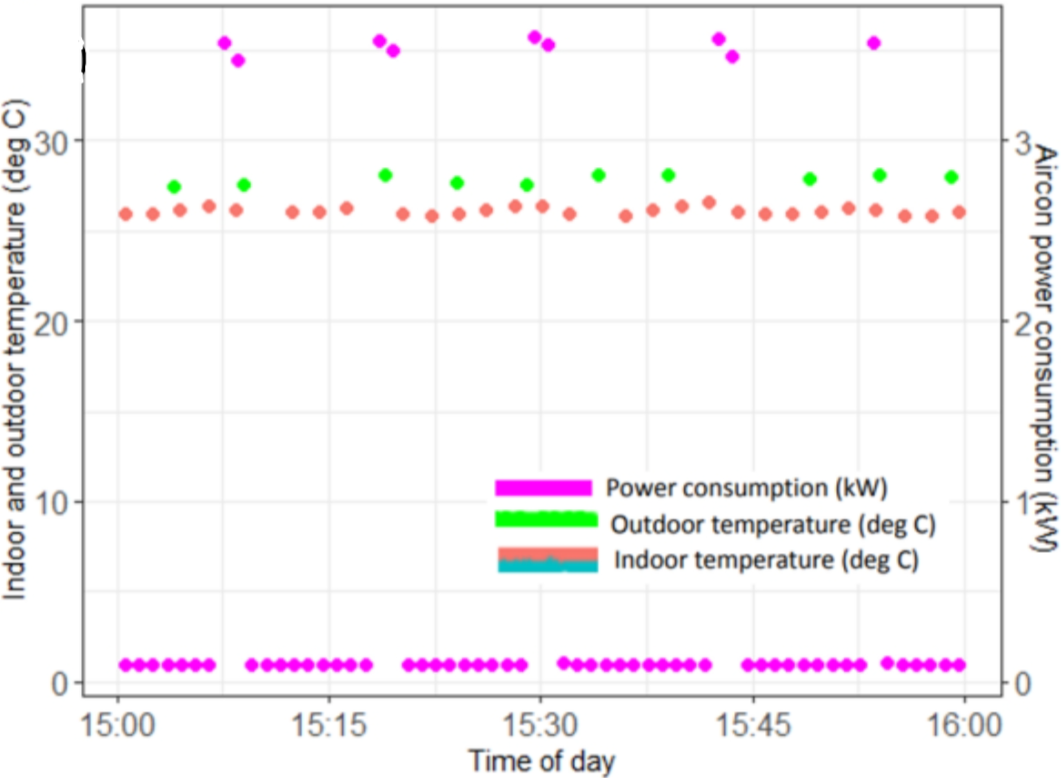
\includegraphics[scale = 0.19]{pic/ac_power_B.png}
        \caption{\footnotesize AC power consumption and ambient temperature in Room A (left) and Room B (right)}
    \end{figure}
\end{frame}

\begin{frame}{Data analysis}
    \begin{columns}
        \column{0.3\textwidth}
        \centering
        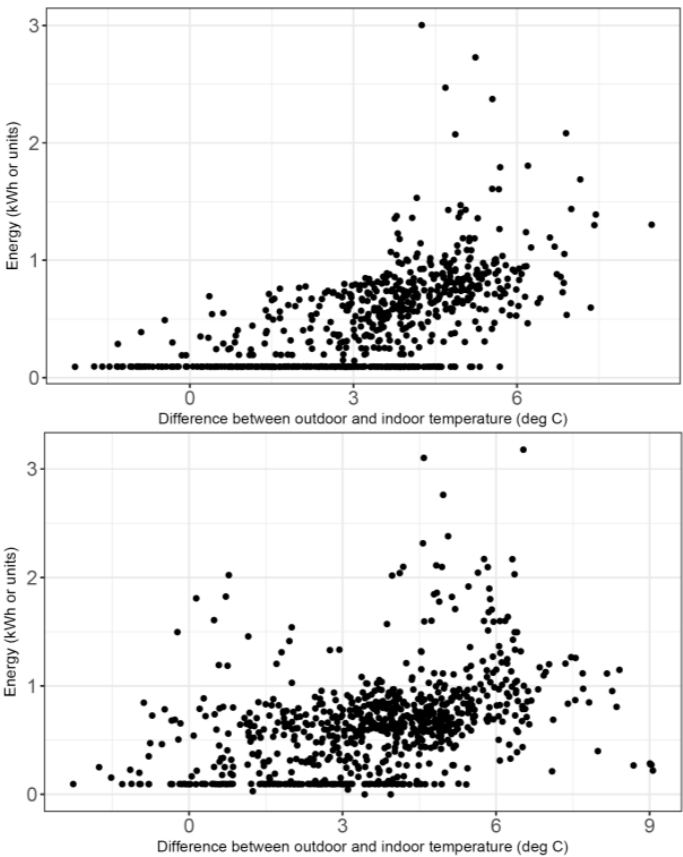
\includegraphics[scale = 0.20]{pic/hourly_energy_consume.png}

        \column{0.3\textwidth}
        \centering
        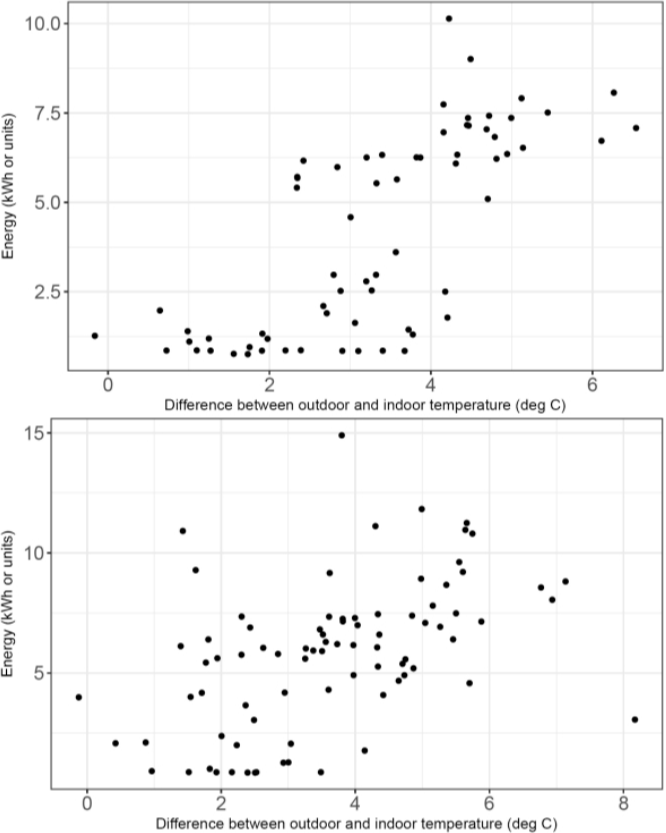
\includegraphics[scale = 0.205]{pic/daily_energy_consume.png}
    \end{columns}
    \begin{figure}
        \caption{\footnotesize Hourly and daily energy consumption w.r.t outdoor-indoor temperature difference}
    \end{figure}
\end{frame}

\begin{frame}{Data analysis}
    \begin{columns}
        \column{0.55\textwidth}
        \begin{table}
            \caption{Daily energy consumption}
            \begin{small}
                \begin{tabular}{c | c | c | c | c}
                    Room & Diff$^1$ & Days$^2$ & Mean$^3$ & STD$^4$ \\
                    \hline
                    \multirow{2}{*}{A}  & 2-3 & 16 & 2.85 & 2.17 \\ 
                                        & 4-5 & 18 & 6.11 & 1.82 \\
                    \hline
                    \multirow{2}{*}{B}  & 2-3 & 18 & 3.79 & 2.54 \\ 
                                        & 4-5 & 21 & 6.89 & 2.32 \\
                \end{tabular}
            \end{small}
            \scriptsize{\\
            \raggedright
                $^1$Outdoor-indoor temperature difference(°C)\\
                $^2$Number of days available for computation\\
                $^3$Average daily energy consumption (kWh)\\
                $^4$Standard deviation of daily energy consumption (kWh)\\
            }
        \end{table}
        \begin{block}{}
            \small{\textit{These infomations help building operator to make the decision to control system for \textbf{reducing} outdoor-indoor \textbf{temperature difference} to \textbf{\textcolor{red}{save energy}}.}}
        \end{block}
        \column{0.45\textwidth}
            \begin{figure}
                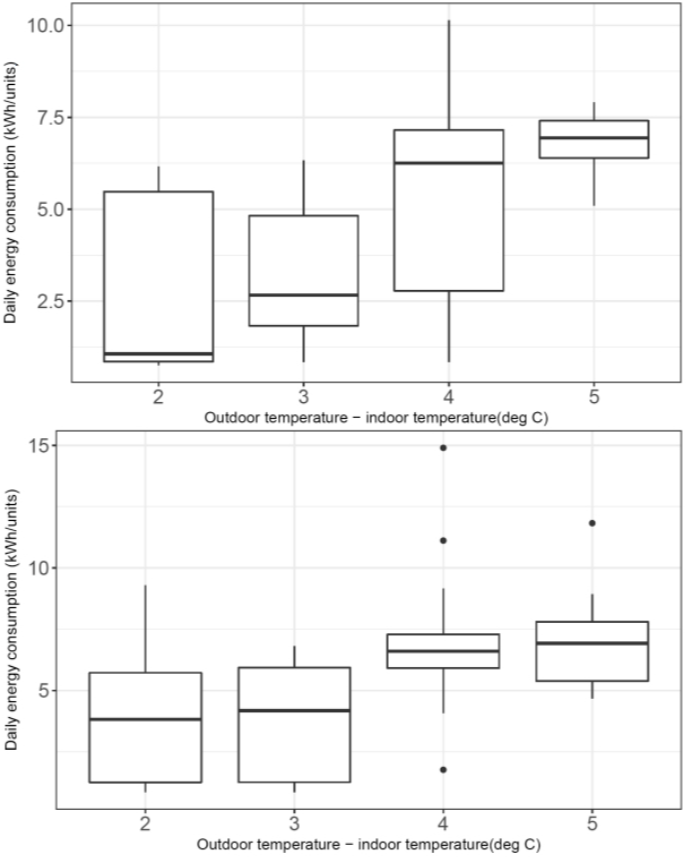
\includegraphics[scale=0.25]{pic/daily_boxplot.png}
                \caption{\footnotesize{Boxplot of daily energy consumption}}
            \end{figure}
    \end{columns}
\end{frame}

\begin{frame}{Data analysis}
    \begin{columns}
        \column{0.5\textwidth}
        \begin{block}
            \small{Energy savings achieved with \textbf{compensated temperature} by personal fan control.}
        \end{block}
        \hspace{1cm}
        \begin{figure}
            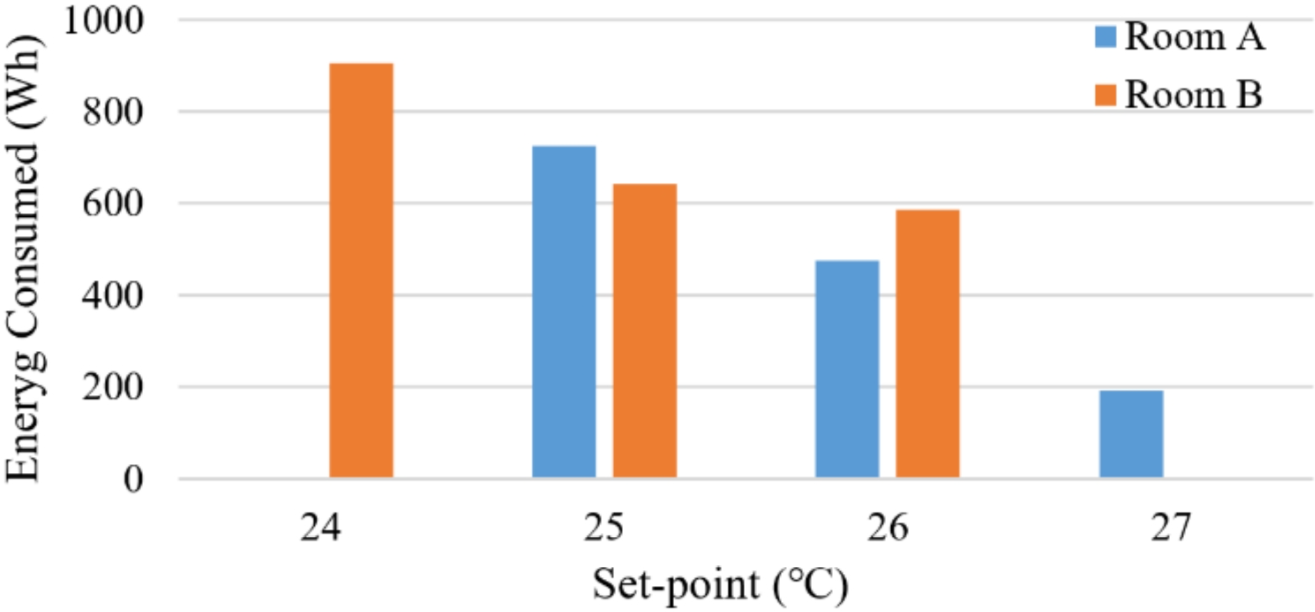
\includegraphics[scale=0.15]{pic/acmv.png}
            \caption{\footnotesize{ACMV energy consumption}}
        \end{figure}
        \column{0.5\textwidth}
        \begin{figure}
            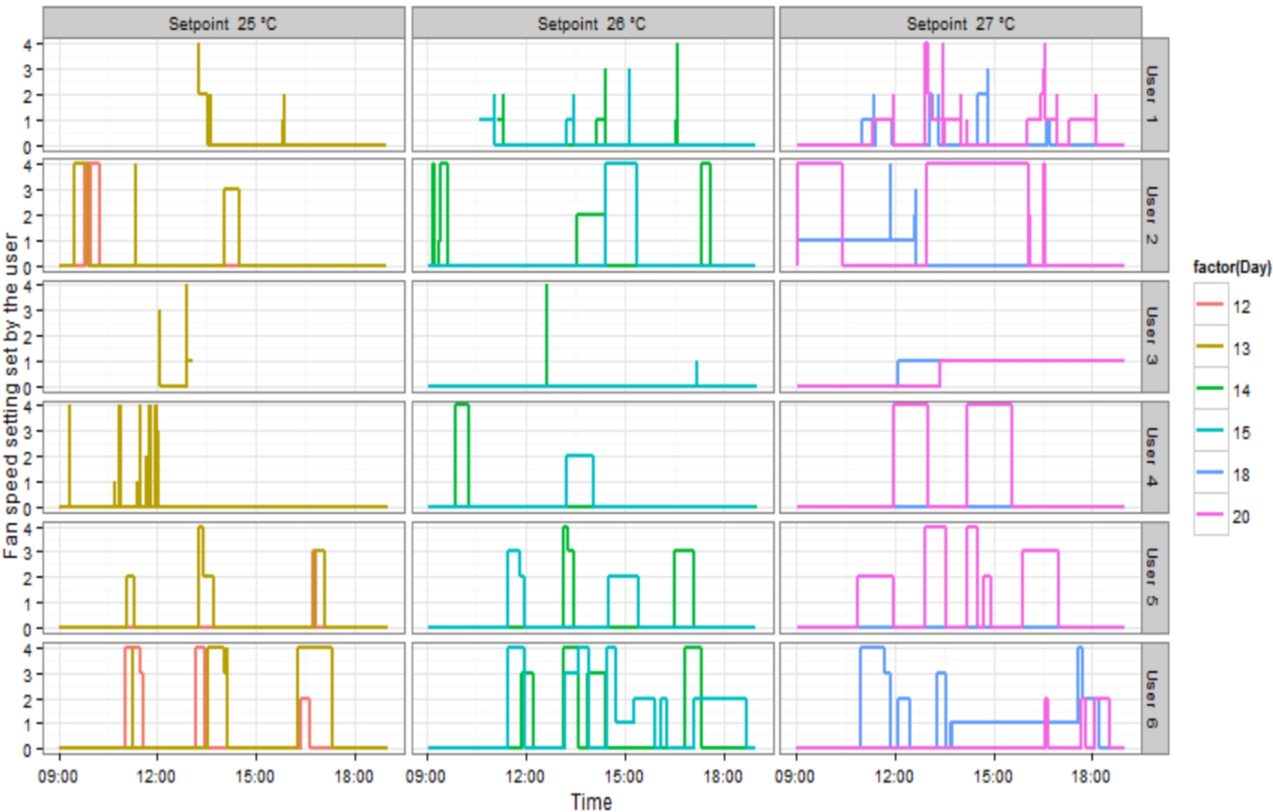
\includegraphics[scale=0.17]{pic/fan_usage.png}
            \caption{\footnotesize{Fan usage data during experiment period}}
        \end{figure}
    \end{columns}
\end{frame}

%=======================================

\section{Conclusion and future work}
\begin{frame}{Conclusion and future work}
    \begin{itemize}[label=\ding{51}]
        \item Demonstrated \textbf{cyber-physical system} for smart building
        \item Performed \textbf{data collection and analysis} of energy usage for air conditioning system
        \item Achieved expectation of \textbf{human comfort} and \textbf{energy savings}
    \end{itemize}
    \hspace{5mm}
    \hspace{5mm}
    \begin{itemize}
        \item[$\blacksquare$] Perform new strategies when considering user-persence and time-varying electricity prices
        \item[$\blacksquare$] Investigate comparsion of energy saving achievable w.r.t other research works
    \end{itemize}
\end{frame}


%==========================

\begin{frame}{References}
    \footnotesize{
    \begin{thebibliography}{99} % Beamer does not support BibTeX so references must be inserted manually as below
        \bibitem[Smith, 2012]{p1} H.D. Chinh, S.S. Shetty, M. Gupta, S.K. Panda (2016)
        \newblock A wireless sensor and actuator network (WSAN) framework for personalized thermal comfort in office buildings
        \newblock \emph{IEEE International Conference on Sustainable Energy Technologies (ICSET), 45 -- 47, Hanoi (2016).}
    \end{thebibliography}
    \begin{thebibliography}{99} % Beamer does not support BibTeX so references must be inserted manually as below
        \bibitem[Smith, 2012]{p1} A. H.-y. Lam, Y. Yuan, and D. Wang (2014)
        \newblock An occupant-participatory approach for thermal comfort enhancement and energy conservation in buildings
        \newblock \emph{5th international conference on Future energy systems, 133 -- 143, ACM (2014).}
    \end{thebibliography}
    }
\end{frame}

%==========================

\begin{frame}
\Huge{\centerline{\textbf{THANK YOU}}}
\end{frame}

%=========================================

\end{document}